\subsection{Savybių atrinkimas}

Klasifikuojant daugiamačius duomenis susiduriame su taip vadinamu dimensiškumo
prakeiksmu (angl. curse of dimentionality). Kai dimensijų skaičius įkopia į
trečią ar ketvirtą eilę naudoti paprastus klasifikavimo algoritmus tampa
nebeefektyvu laiko atžvilgiu. Vienas iš būdų kovoti su dimensiškumo prakeiksmu
yra naudoti vienokius ar kitokius savybių skaičiaus mažinimo metodus. Šiame
darbe nagrinėsiu savybių pasirinkimo pagal keletos kriterijų suliejimą metodą
(angl.
feature selection based on multicriterion fusion)\cite{5611484}, bei
stabilių savybių grupių išskyrimo metodą\cite{Loscalzo:2009:CGS:1557019.1557084}.

\subsubsection{Savybių pasirinkimo pagal keletos kriterijų suliejimą metodas}

Šio metodo esmė yra panaudoti kelis savybių atrinkimo metodus suliejant jų
rezultatus į vieną bendrą rezultatą. Kodėl naudinga sulieti keletą savybių
atrinkimo metodų? Sulieti keletą savybių atrinkimo metodų naudinga, nes
pavieniai savybių atrinkimo metodai be to, kad turi savitų privalumų, visada
turi ir savo silnybių, pavyzdžiui, jautrumas išimtims (angl. outliers), negali
rasti savybių tarpusavio priklausomybių, etc. Suliejant keletą skirtingų metodų
suliejamos gerosios pavienių savybių atrinkimo metodų savybės, taip
kompensuojant algoritmų silpnybes.

Galima pavienių savybių atrankos rezultatus sulieti pagal šias suliejimo
strategijas:
\begin{enumerate}
  \item Suliejimas pagal svorius
  \item Suliejimas pagal reitingus (angl. rank)
  \item Sulieti ir pagal svorius ir pagal reitingus
\end{enumerate}

Suliejimo pagal svorius būdu būtinai reikia atlikti svorių normalizavimą. Kitu
atveju savybių įvertinimo metodai bus nepalyginami. Pirmajame paveikslėlyje
nenormalizuotų svorių skiriasi netgi intervalai. Antrajame paveikslėlyje matoma,
kad net ir normalizavus svorius gana stipriai skiriasi svorių kvartiliai.

\begin{figure}[htb]
\begin{center}
\leavevmode
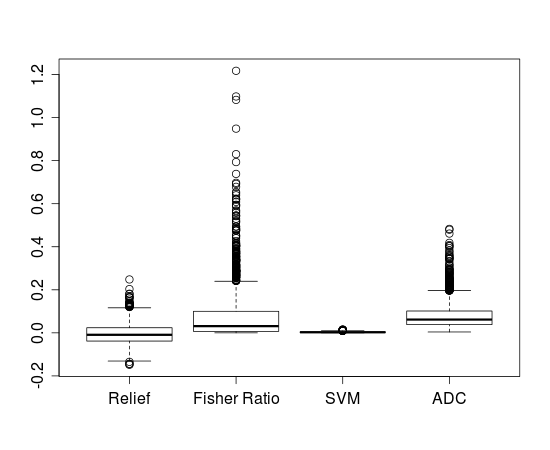
\includegraphics[width=0.5\textwidth]{images/boxplot_colon_all.png}
\end{center}
\caption{Pavienių savybių atrinkimo metodų nenormalizuotas svorių
pasiskirstymas.}
\label{fig:flash}
\end{figure}

\begin{figure}[htb]
\begin{center}
\leavevmode
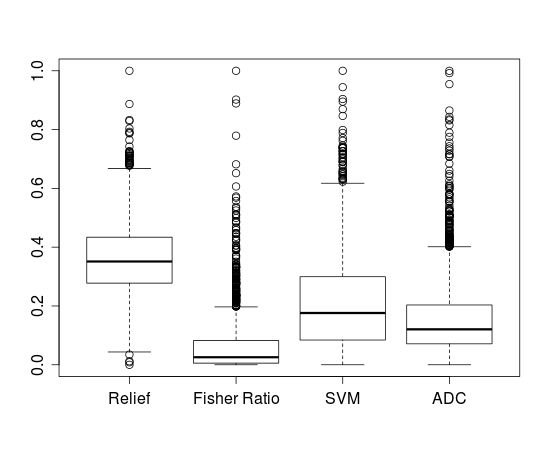
\includegraphics[width=0.5\textwidth]{images/boxplot_colon_all_normalized.png}
\end{center}
\caption{Pavienių savybių atrinkimo metodų normalizuotas svorių
pasiskirstymas.}
\label{fig:flash}
\end{figure}

Suliejimo pagal reitingus metodas nereikalauja normalizavimo, nes tiesiog imame
savybių svorių įverčius ir juos išrykiuojame mažėjimo tvarka - išreitinguojame.

Savybių įverčių pagal svorius ir reitingus metodas vyksta dviem žingsniais:
\begin{enumerate}
  \item suliejame savybes pagal svorius ir taip gauname vieną savybių reitingą,
  kurį prijungiame prie kitų savybių reitingų;
  \item reitinguojame savybes pagal visus turimus pavienius reitingus.
\end{enumerate} 
